\chapter{Resultados}

Para a execu\c{c}\~ao do projeto, algumas etapas de desenvolvimento tiveram de ser seguidas: familiariza\c{c}\~ao com o sistema, estudo dos módulos envolvidos, leitura dos requisitos, elabora\c{c}\~ao de documento descrevendo todo o processo de implementa\c{c}\~ao e relacionamento com os diversos m\'odulos, implementa\c{c}\~ao e testes.

\section{Atividades do Projeto}
\markright{\thesection ~~~ Metodologia}
\label{metodo3}

\section {Requisitos do Sistema}
\markright{\thesection ~~~ Requisitos}
\label{req}






\begin{figure}[htbp]
\centering
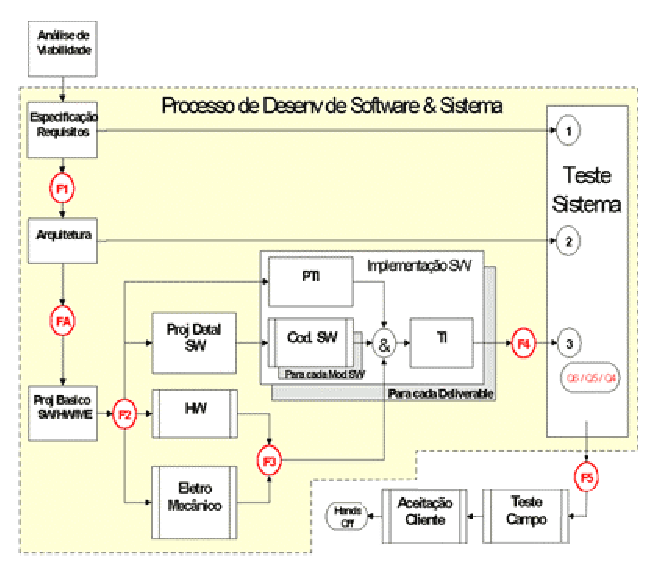
\includegraphics[scale=1.2]{Resultados/ciclodesenvolvimento.eps}
\caption{Ciclo de desenvolvimento de um projeto}
\label{CicloDesenvolvimento}
\end{figure}

Para referenciar a Figura \ref{CicloDesenvolvimento}, veja arquivo .tex.



Aqui começa uma sub-seção.


\section{Desenvolvimeto e Implementação}

Aqui começa outra seção.

Para inserir a tabela abaixo, veja arquivo .tex.

\begin{table}
\centering
\begin{tabular}{|l|l|}\hline
		1.Uso do serviço & Para o assinante rastrear uma chamada, ele deverá tirar\\ 
										 & o telefone do gancho, esperar pelo tom de discagem e então \\
										 & discar o código de acesso ao serviço. \\ \hline
		2.Processamento  & Caso o assinante tenha acesso ao serviço SRUC, ele deverá  \\			
		  do serviço 		 & ouvir um anúncio, ao discar o código de acesso, explicando \\
									   & que o serviço SRUC foi acessado. Dessa forma, se os dados \\
									   & a serem rastreados forem suficientes, o sistema deverá \\
									   & fornecer uma mensagem de confirmação de \\
									   & serviço realizado \\ \hline
		3. Ativação da   		& A ativação do serviço somente será válida \\
			 última chamada   & para a última chamada recebida. \\ 
			 recebida				 	& \\ \hline
		4. Mais de uma   		& Se o assinante tentar ativar o serviço para a mesma chamada \\
			 ativação para 	 	& ele deverá ouvir novamente o anúncio de serviço realizado, mas \\
			 a mesma chamada	& não irá gravar os dados novamente \\ \hline
		5. Número privado 	& O sistema deverá mostrar o número do assinante chamador \\
			 do assinante A  	& mesmo que este não possa ser mostrado. \\ \hline
		6. Chamadas  				& Para que o serviço possa valer para chamadas intercentrais \\
			 intercentrais		& a central deverá utilizar a sinalização SS7, e o número do \\
												& assinante A será obtido pela mensagem IAM. \\ \hline
		7. Informações de 	& Um \textit{trace} do serviço deverá possuir os seguintes itens:\\
			 um registro			& Número do assinante A \\
												& Hora da chamada recebida\\
												& Data da chamada recebida\\
												& Número do assinante B\\
												& Hora da solicitação do serviço\\
												& Data da solicitação do serviço\\
												& Dados sobre rota para chamadas intercentrais \\ \hline
		8. Tratamento para 	& Se um assinante discar o código de acesso ao \\
		   assinante sem 		& serviço, a central deverá fornecer tratamento padrão \\
			 serviço					& de acesso negado. \\ \hline
		9. Tipos de 				& A central deve permitir que o assinante com o serviço \\
		   telefones				& possua tanto DTMF quando Dial Pulse \\ \hline
		10. Comandos do 		& O sistema supervisório conectado à central deverá \\
		    sistema 				& disponibilizar um  comando para que o operador possa  \\
		    supervisório		& descarregar o arquivo com os \textit{traces} das chamadas \\
		    								& para os diversos assinantes de uma central. \\
												& Um comando para visualizar os \textit{traces} também será necessário. \\ \hline
		\end{tabular}
	\caption{Requisitos do Serviço SRUC}
	\label{tab:RequisitosDoServiçoSRUC}
\end{table}

Aqui você referencia a tabela: a Tabela \ref{tab:RequisitosDoServiçoSRUC} explicita os pontos mais relevantes na implementação do SRUC.

\section{Testes}

\section{Resumo do Capítulo}
\markright{\thesection ~~~ Metodologia}
\label{metodo4}
Esse capítulo pode ser dividido em duas partes $	f=ma $ blaba \cite{bel/00}
 
\begin{gather}
	f=ma\\
	x=2\\
\end{gather}

\begin{align}
	f=ma\\
	x=2\\
\end{align}

\begin{eqnarray}
	f=ma\\
	x=2\nonumber\\
\end{eqnarray}


\clearpage